\documentclass{article}

\usepackage[utf8]{inputenc}
\usepackage[T1]{fontenc}
\usepackage{polski}

\usepackage{lastpage}
\usepackage{graphicx} 

\usepackage{caption}

\captionsetup[figure]{name={Rysunek}}
\hoffset=-1.0cm

\usepackage{fancyhdr}
\pagestyle{fancy}
\fancyhf{}
\rfoot{Strona \thepage \hspace{1pt} z \pageref{LastPage}}

\title{Symulacja pracy z Tablicą Kanban - aplikacja webowa - specyfikacja funkcjonalna
przed wykonaniem projektu}
\author{}
\date{}

\begin{document}
\maketitle

\begin{flushright}
\par
\vfill
\par
Wykonał: Bartosz Zakrzewski

Data: 04.04.2021

\end{flushright}
\thispagestyle{empty}

% \newpage

\tableofcontents

% \newpage

\section{Cel dokumentu}
Dokument ma na celu przedstawić funkcje jakie projektowana aplikacja webowa ma spełnić. 
Zostanie w nim pokazany poglądowy wygląd strony.

\section{Cel projektu}
Celem projektu jest stworzenie aplikacji webowej, która ma zasymulować przebieg pracy z Tablicą Kanban. \\
Tablica Kanban to narzędzie wykorzystywane w zarządzaniu projektami, która zwykle przedstawia przebieg prac w postaci zadań, które przemieszcza się między kilkoma kolumnami.

\section{Wymagania funkcjonalne}
\begin{itemize}
    \item Definiowanie limitów ilości zadań w poszczególnej kolumnie;
    \item Oznaczanie wykonanej pracy - wypełnianie progresu (np. w postaci checkboxów) wewnątrz danego zadania/taska;
    \item Mechanizm rzucania kostką 1-5 - jest to generowanie produktywności danego dnia dla danej osoby;
    \item Generowanie blokerów - daje znać użytkownikowi, że z zadaniem są trudności; 
    \item Blokera da się usunąć np. wykorzystując punkty progresu;
    \item Przypisywanie osoby do zadania (oznaczenie kolorystyczne);
    \item 3 rodzaje taska: Zwykły, Urgent, Fixed Date (nazwa i np. dodatkowo kolorystyka);
\end{itemize}

\section{Dodatkowe wymagania funkcjonalne}
Po zakończeniu pracy nad podstawowymi zadaniami projekt można rozszerzyć o następujące zagadnienia (w danej kolejności):

\begin{enumerate}
    \item Zadanie ma pole do wpisania dnia początkowego i końcowego;
    \item Ustalanie prawdopodobieństwa generowania blokerów;
    \item Symulacja jest oparta na historiach opisujących kolejne dni pracy;
    \item Definiowanie własnych kolumn;
    \item Definiowanie limitów na kilka kolumn;
    \item Wiele osób używa tablicy naraz;
\end{enumerate}

\clearpage

\section{Wygląd strony}
Warto zaznaczyć, że projekt jest inspirowany podobną aplikacją webową stworzoną przez Okaloa (https://www.okaloa.com/).

 \begin{figure} [hbt!]
        \centering
        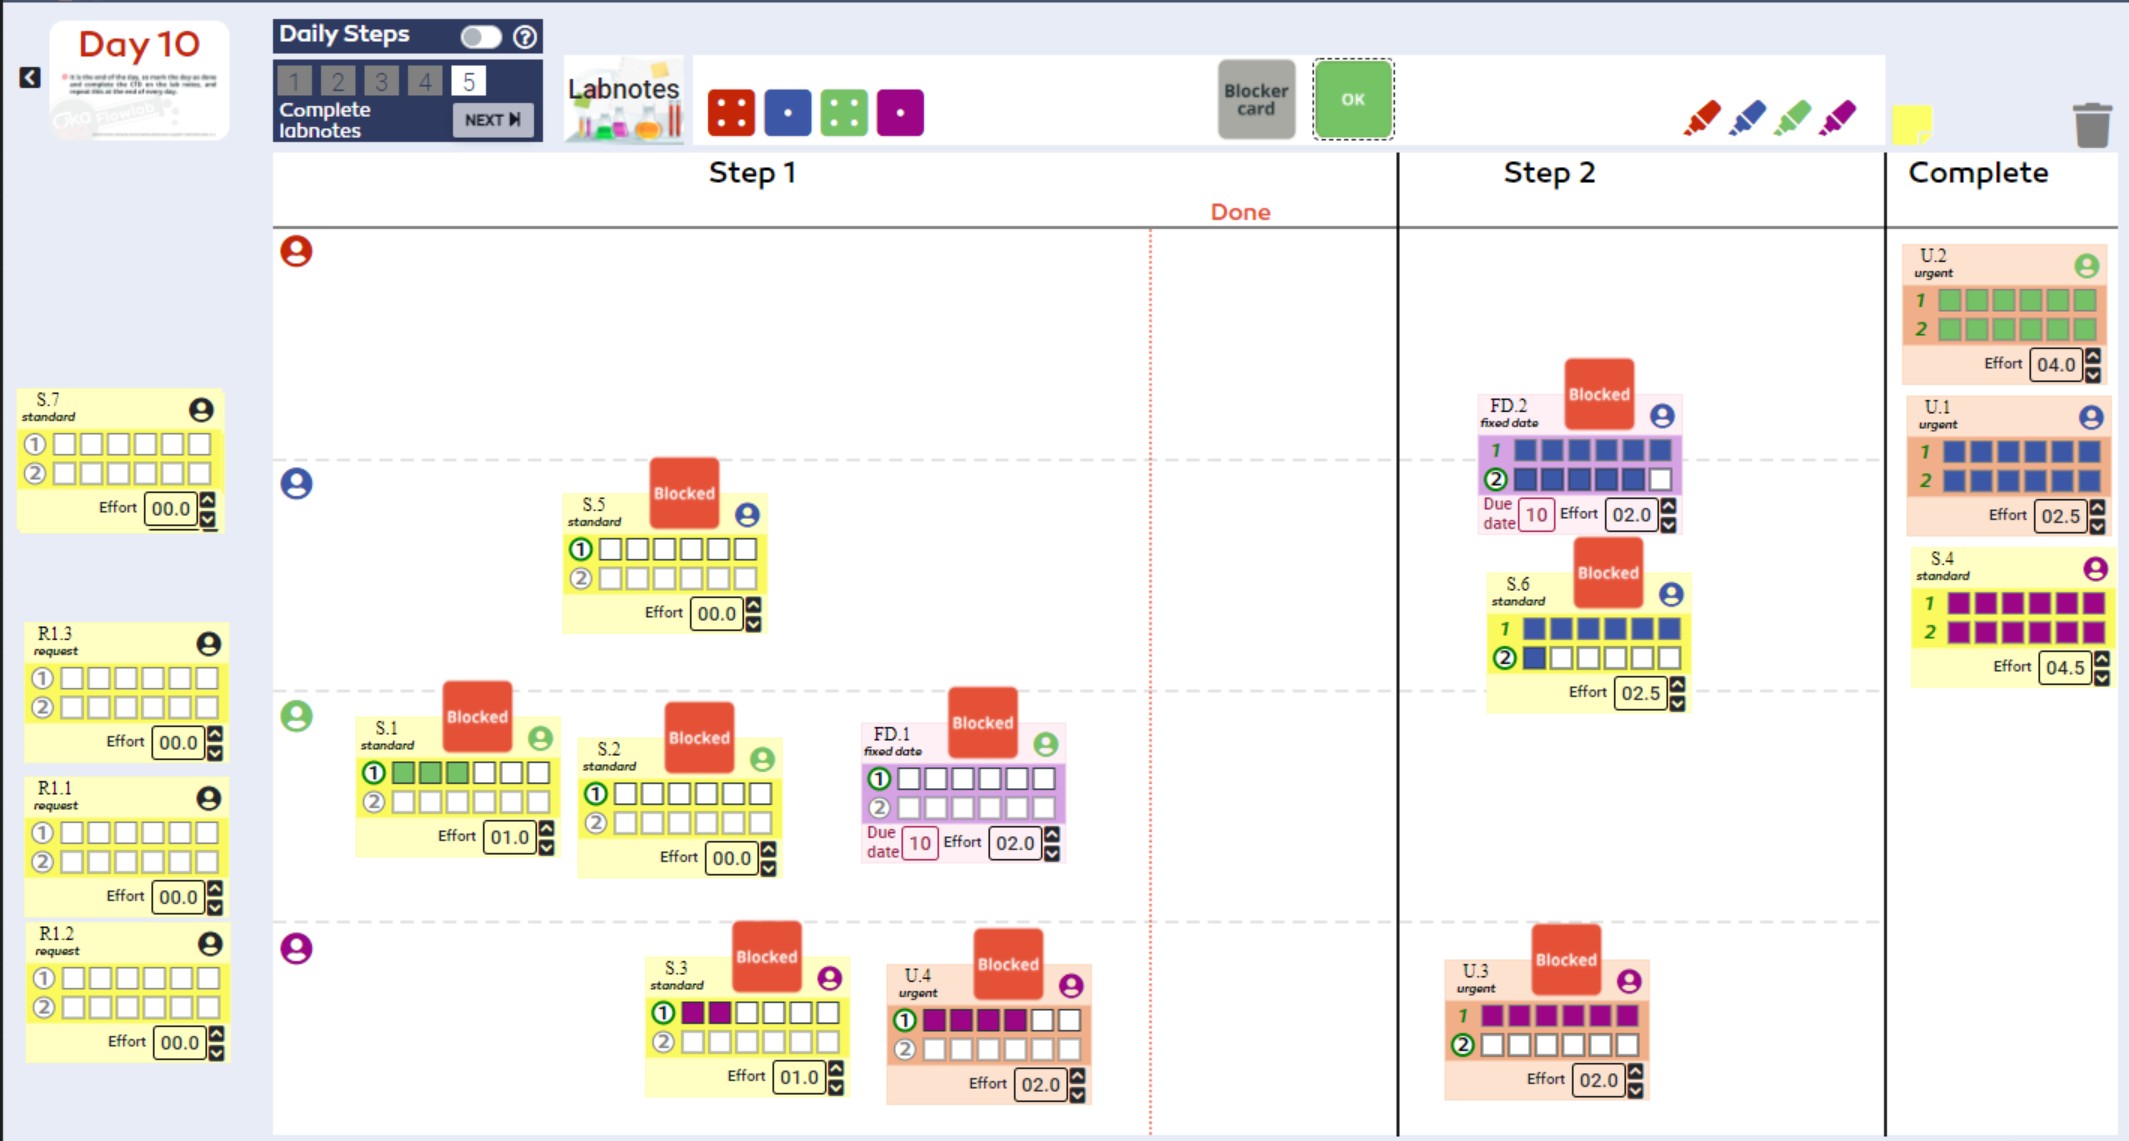
\includegraphics[width=16cm]{img/kanban_by_okaloa.png}
      \captionof{figure}{Okaloa Flowlab Kanban Board}
    \end{figure}
    
\end{document}
